\chapter{Related Work}
\label{ch:relatedwork}

Automated fault localization in general and more specifically spectrum-based
fault localization have extensive literature exploring the different approaches
to facilitate debugging and increase developer efficiency. Considering that
AFLuent relies on many concepts developed by this literature, this section will
explore and discuss how past work shapes AFLuent. Several sections are created
for specific areas of literature.

\section{Automated Fault Localization}
\label{sec:AFLlit}

Survey papers are one of the many ways that assist in better
understanding and having a wide collection of the existing
literature surrounding automated fault localization (AFL).
Wong et al. \cite{wong2016survey} explores the variety of AFL approaches and
surveys research completed in that area between 1977 and 2014. The survey paper finds and
discusses more than 334 different papers in many approaches in AFL.

\begin{figure}[!htb]
	\begin{center}
		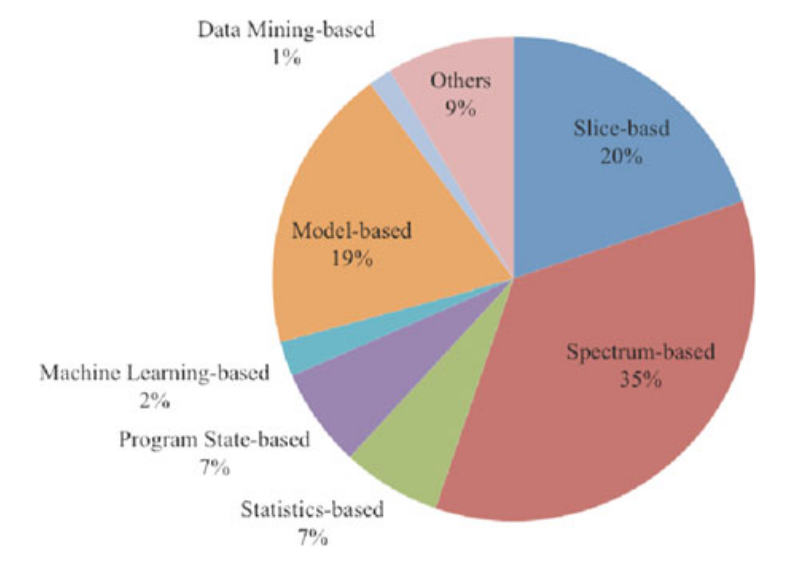
\includegraphics[width=10cm]{wong_pie_chart.png}
		\caption{\label{fig:wong_breakdown} AFL papers found by Wong et al. \cite{wong2016survey}}
	\end{center}
\end{figure}

A breakdown of the found research is shown in Figure \ref{fig:wong_breakdown}, where the
majority of found papers are focused on Spectrum-Based Fault Localization (SBFL).
Overall this research provides a great
starting point to find and compare the different types and approaches of AFL.
Another benefit of these resources is that
Wong et al. \cite{wong2016survey} expands on the types of SBFL
and reviews key literature that contributes to show the benefits and drawbacks of
each approach.

Another insightful survey paper is by Idrees Sarhan et. al \cite{sarhan2022Challenges}
where he analyzes the main challenges in SBFL and some of
the major obstacles that other literature attempts to tackle. AFLuent addresses
two of the issues listed in this survey study, specifically element ties and
division by zero. But many other challenges such as test flakiness, single vs.
multiple bugs, and many others remain unaddressed.

\subsection{SBFL Approaches}
\label{subsec:sbfl}

\subsubsection{Similarity Coefficient Based Technique}
\label{subsubsec:coefficient_based}

One of the most relevant SBFL techniques described by Wong et al.
\cite{wong2016survey} is similarity coefficient based ones. Generally, these approaches
seek to quantify how close ``the execution pattern of a statement is to the
failure pattern of all test cases'', where the closer they are the more
likely that this statement to contain the error. In order to create a
measurement of closeness, several equations have been developed and evaluated by
past literature. Figure \ref{fig:sbfl_eq} shows some of the equations reviewed by
Wong et al in, however, more popular formulas have been developed that
required the developer to analyze less code before finding the fault. Despite
the existence of many Similarity Coefficient formulas, Yoo et al.
\cite{yoo2014no} concludes in an extensive evaluation study that there is no
formula that outperforms all others in all circumstances. With that in mind,
AFLuent gives the user the option to choose which approach to use and includes
a performance evaluation of each.

\begin{figure}[!htb]
	\begin{center}
		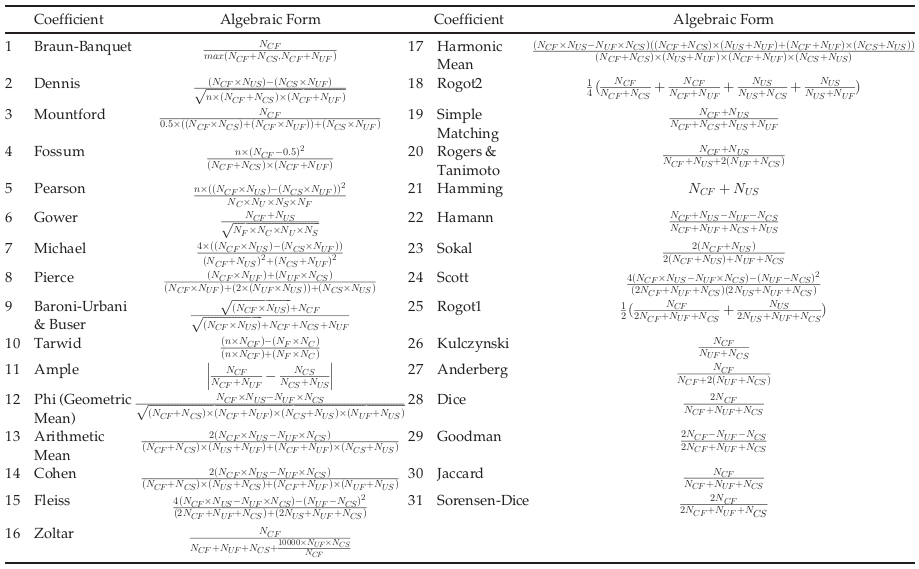
\includegraphics[width=\textwidth]{sfl_table.png}
		\caption{\label{fig:sbfl_eq} Coefficient Based Formulas \cite{wong2016survey}}
	\end{center}
\end{figure}

\subsubsection{Tarantula}
\label{subsubsec:tarantula_lit}

Starting off with the Tarantula formula (figure \ref{fig:tarantulaEquation}), it's
one of the foundational equations that was introduced to attempt to visualize
suspicious statements using color ranges \cite{jones2002viz,
Jones2005TarantulaEval}. A tool using this equation was also implemented in Java
in order to scan code and assign colors to statements based on their
suspiciousness. The equation for Tarantula is made of two main ratios, the first
one being the number of failed tests that cover the element divided by the total
number of failed tests (\(\frac{\textbf{N$_{CF}$}}{\textbf{N$_{CF}$ +
\textbf{N$_{UF}$}}}\)). The other ratio used is number of passing tests that
cover the element divided by total number of passing tests
(\(\frac{\textbf{N$_{CS}$}}{\textbf{N$_{CS}$}+\textbf{N$_{US}$}}\)).
The equation is then assembled as seen in figure \ref{fig:tarantulaEquation}.
To better understand how the equation works, we can look at the important terms
that have the largest influence in changing the output.The number of failed
tests that cover the element is clearly the main influencer here because it's
what causes the numerator to grow larger. This means that an increase in failed
tests that cover the element cause an increase in suspiciousness. Additionally,
a decrease in the number of failing tests that do not cover the element also
increases suspiciousness. Considering these two points, Tarantula gives a better
indicator of suspiciousness when there are fewer failures in tests covering
elements not under inspection. In addition to the logical analysis of the
equation previous works provide an empirical evaluation of Tarantula in
comparison to other formulas. Jones et al. \cite{Jones2005TarantulaEval}
compares the effectiveness and efficiency of Tarantula to techniques such as Set Union, Set
Intersection, and Nearest Neighbor. The results demonstrate that Tarantula
outperformed the other Techniques where it provided better guidance to the
developer. Using Tarantula a developer would need to manually
inspect fewer elements of the program compared to when using other approaches.

Another variation of Tarantula is also introduced in \cite{debroy2010grouping},
where grouping of suspicious elements is used to provide a better guide for
developers. In this modification, ``statements that are executed by the same
number of failed test cases are grouped together'', then suspiciousness scores
are used to sort elements within each group. By doing so, two layers of sorting
exist, the first one based on the number of failed tests covering the element,
and then the suspiciousness scores. The empirical results in Debroy et al.
\cite{debroy2010grouping} show a statistically significant improvement provided
by this grouping technique where the developer needs to review less elements and
more faults are accurately detected. While Debroy et al. only applied the
grouping technique to Tarantula and a neural network-based approach, it could be
extended to include other similarity coefficient based techniques.

Overall, while other formulas outperform Tarantula as will be discussed,
incorporating this equation in AFLuent offers a starting point and a point of
comparison to other equations. One of the goals of AFLuent is to give the user
the ability to choose their most fitting approach to localize faults, and it's
useful to include Tarantula as one of the available options.

\subsubsection{Ochiai}
\label{subsubsec:ochiai_lit}

Ochiai is another similarity coefficient formula for SBFL that uses code
coverage information and test output to produce a suspiciousness score.
Originally used in computing genetic similarity in molecular biology and
evaluated in Abreu et al. \cite{Abreu2006Ochiai}, the equation for this approach
is shown in fog.\ref{fig:ochiaiEquation}. Similar to Tarantula, the number of
failing test cases that execute an element are the main factor in increasing
suspiciousness. The formula uses similar terms as Tarantula such as total number
of tests that cover the element, unlike Tarantula, however, it does not consider
successful tests that do not cover the element.
Papers such as \cite{Abreu2006Ochiai,ABREU20091780} also evaluate the
performance of Ochiai in comparison to others such as Tarantula, AMPLE, and
Jaccard. Another evaluation of Ochiai is done by Le et al. \cite{le2013theory}
where it was found to have a statistically significant improvement when compared
to Tarantula. The paper demonstrates that on average developers only need to
inspect 21.02\% of the source code before finding the fault.
AFLuent includes an implementation and evaluation of Ochiai to
validate that it performs as expected compared to the Tarantula technique.
Additionally, considering that Ochiai is considered a fairly accurate and
effective formula to detect faults, AFLuent takes advantage of the performance
it offers.

\begin{figure}[!htb]
	\begin{center}
		\begin{equation}
			Ochiai2(element) = \frac{\textbf{N$_{CF}$}\cdot{\textbf{N$_{US}$}}}{\sqrt{(\textbf{N$_{CF}$}  + \textbf{N$_{CS}$}) \cdot (\textbf{N$_{US}$}  + \textbf{N$_{UF}$}) \cdot (\textbf{N$_{CF}$}  + \textbf{N$_{UF}$}) \cdot (\textbf{N$_{CS}$}  + \textbf{N$_{US}$})}}
		\end{equation}
		\caption{\label{fig:ochiai2Equation} Ochiai2 Equation\cite{wong2016survey}}
	\end{center}
\end{figure}

In addition to the Ochiai formula in figure \ref{fig:ochiaiEquation}, another
variation of Ochiai is identified and evaluated by \cite{naish2011model}. The
formula for Ochiai2 is shown in \ref{fig:ochiai2Equation} and it takes into
consideration all the possible outcomes of unit test coverage. Overall, this
variation is included in AFLuent to compare the performance between Ochiai2 and
the original formula and see if it provides an improvement in effectiveness.
Both Ochiai and Ochiai2 are relevant similarity coefficient-based approaches
that add variety to AFLuent and allow a representative evaluation of the tool
that takes in many different approaches..

\subsubsection{DStar}
\label{subsubsec:dstar_lit}

DStar (also written as D*) is another SPFL technique that utilizes code coverage
information of a program to locate and rank faults. The equation for this
approach can be found in figure \ref{fig:dstarEquation}. Wong et al.
\cite{Wong2014DStar} introduce and extensively evaluate this approach in a 2014
paper that demonstrate its effectiveness compared to other formulas. In the
process of constructing D*, the paper lists the factors involved in determining
suspiciousness of an element. The principles are as follows:
\begin{enumerate}
	\item Suspiciousness is directly proportional to the number of failed tests
	covering the element.
	\item Suspiciousness is inversely proportional to the number of successful tests
	covering the element.
	\item Suspiciousness is inversely proportional to the number of failed tests
	that do not cover the element.
	\item The number of failed tests covering the element should have the most
	weight in determining suspiciousness.
\end{enumerate}

Considering that multiplying \(\textbf{N$_{CF}$}\) by a constant to increase its
weight will not affect the ranking of statements, the authors argue that
raising \(\textbf{N$_{CF}$}\) to a value * greater than
or equal to 1 would be more appropriate in increasing the weight of this
variable. The study continues by illustrating how increasing the value of *
produces more clear rankings that facilitate the debugging process by requiring
the developer to examine less elements in both the best and worst case. However,
the authors also point out that this benefit of increasing the value of * levels
off at a certain point depending on the size of the program under analysis.
The paper concludes by reviewing performance results showing that D* is more
effective than the previously discussed formulas (Tarantula, Ochiai, and
Ochiai2). With that in mind, D* offers the latest and most effective formula to
calculate suspiciousness compared to all others included in this research.
AFLuent implements D* to validate this step up in effectiveness in the context of
Python projects and gives the user the ability to use it.

\subsection{Combining Approaches}
\label{subsec:combining_approaches}

While AFLuent only relies on SBFL approaches in its implementations, it's
useful to explore other methodologies that could assist in the debugging
process. This creates a guide for potential extension of AFLuent and
provides a way to fill in the shortcomings of AFLuent. Xuan et al. explores the
possibility of combining several SBFL metrics of fault localization and
introducing a machine learning model to assist with the ranking
\cite{Xuan2014Combine}. While AFLuent does not support this approach, Xuan et
al. shows some promising results that could potentially uncover performance
improvements in fault localization. There are many tricky aspects of this
research, especially that it suggests training a machine learning model to
assist with ranking. Depending on the data used to train the model, the results
could be very different. Overall, while AFLuent does not use machine learning,
this research provides a great idea for future work and improvements.

Another proposed extension to the existing SBFL work is studied by Wang et al.
\cite{Wang2011Search} where similar to the previous work, a ``Search-Based
Composition Engine'' is trained using a set of coverage information as well as
locations of existing bugs. Additionally, it creates a composite equation using
multiple coefficient-based formulas and their weights as part of the engine. The
resulting evaluation shows that this approach does, in fact, outperform standard
formulas like Tarantula and Ochiai.

Overall, while these works are somewhat out of scope of AFLuent since they use
different techniques, they have the same intention in optimizing the debugging
process and reducing its cost. The research discussed in this section could
potentially get used to extend the functionality of AFLuent where a model/engine
is trained through the feedback of users which allows them to use it later in
their debugging efforts.

\subsection{Acknowledging Problems}
\label{subsec:acknowledging_problems}

With the multitude of approaches and formulas to use in SBFL, various criticisms
are brought up for each proposed research. Some research even suggests that SBFL
and AFL in general is not effective for all developers \cite{parnin}. In a survey study, Wong et al.
\cite{wong2016survey} identifies a series of issues and concerns surrounding
SBFL in general. The main one being the central problem of giving failed and
successful tests accurate weights in order to produce a meaningful
suspiciousness score and reduce the potential for ties. Another identified
concern is the assumption that a well written and extensive test suite exists
for the program under examinations but more specifically the assumption SBFL approaches tend to make by
considering passing test cases indicators of error absence. In many instances,
test cases themselves could contain bugs causing them to produce inaccurate results. Existing literature
on both of these concerns exist and it's required to consider this criticism in
the development of AFLuent.

One of the brought up concerns of SBFL is the inclusion of passed program
spectra in calculating suspiciousness of an element. Xie et al.
\cite{xie2010isolating} argue that while a failed program test case does
indicate the presence of an error in a passed program spectra/test data, ``is not
guaranteed to be absolutely free of any faulty statement''. With that in mind,
passed test information alone does not give reliable results on elements
suspiciousness. The proposed approach to mitigate this problem is to organize
program entities into two main groups, those who have been ``activated'' at
least once by a failed program spectra, and ``clean'' ones, which have not at
all. The research continues by experimenting with this approach and presenting
results that showed some signs of improvement on existing SBFL formulas.
Overall, this research provides a way to address inaccuracies with AFLuent and
assists in expanding the project beyond simple calculations based on formulas.

Another concern with the use of SBFL to debug programs is the possibility of
having equal suspiciousness scores assigned to multiple statements. These ties
hinder the debugging process and present the developer with a dilemma. Which
element should be inspected first? they're equally suspicious! This problem
becomes more significant when only one of the tied elements actually contains the
fault. A study by Xu et al. \cite{xu2011ties} recognizes this problem and
expands on the different outcomes. In the best case, the developer picks the
statement containing the fault as their first choice and finds the error right
after. However, the worst case would require the developer to examine every tied
element before reaching the one containing the fault. The research continues by
showing that ties in calculated suspiciousness scores are frequent no matter the
chosen formula. Other contributions of this research include strategies to break
ties and facilitate suspiciousness ranking between elements. The research
concludes by presenting that the tie breaking strategies were impactful in
reducing the number of found ties in Tarantula and Ochiai approaches.

\section{Existing Tools}
\label{sec:existing_tools}

Some tools that perform SBFL have already been proposed and implemented. While
they tend to be standalone applications that operate differently than AFLuent,
it's important to explore the way these applications interact with the user and
show output. Zoltar \cite{janssen2009zoltar} is a standalone tool for C/C++
programs that offers a
graphical user interface for users to view program spectra and calculate
suspiciousness scores using various techniques. The tool also uses the hue
concept developed by an early study that proposes Tarantula \cite{jones2002viz}.
By color coding statements based on their rank and suspiciousness scores, Zoltar
simplifies the user interaction by making it clear which statement is the most
likely to be faulty. While AFLuent lives and runs in a terminal window, it does
utilize color coding elements in its output to increase output readability and
facilitate user interaction. Additionally, AFLuent solves some of the problems
present with Zoltar by existing as a Pytest plugin, which gives it easy access
to program spectra such as test results and statement coverage.

\begin{figure}[!htb]
	\begin{center}
		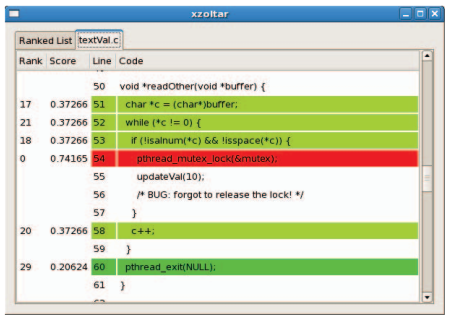
\includegraphics[width=6cm]{zoltar.png}
		\caption{\label{fig:zoltar} Example of Zoltar Interface \cite{janssen2009zoltar}}
	\end{center}
\end{figure}

In contrast to Zoltar, which was used to analyze programs written in C and C++,
CharmFL, is a Python tool that performs SBFL to identify faults. Sarhan et al.
\cite{sarhan2021charmfl} introduce CharmFL in a study that
discusses its features and implementation. The study recognizes the need for
SBFL tools to assist Python developers since it has become a very popular
language. Additionally, it presents CharmFL as a plugin for the popular IDE and
text editor PyCharm. Similar to AFLuent, it uses the Pytest framework to collect
program spectra and calculates suspiciousness scores using Tarantula, Ochiai,
and DStar approaches. Overall, CharmFL has many similarities with AFLuent, but
it's also less accessible considering that it's a PyCharm plugin which is not
used by every developer. Overall, the implementation of CharmFL provides an
inspiration for AFLuent and encourages improvements where CharmFL may fall
short.

\begin{figure}[!htb]
	\begin{center}
		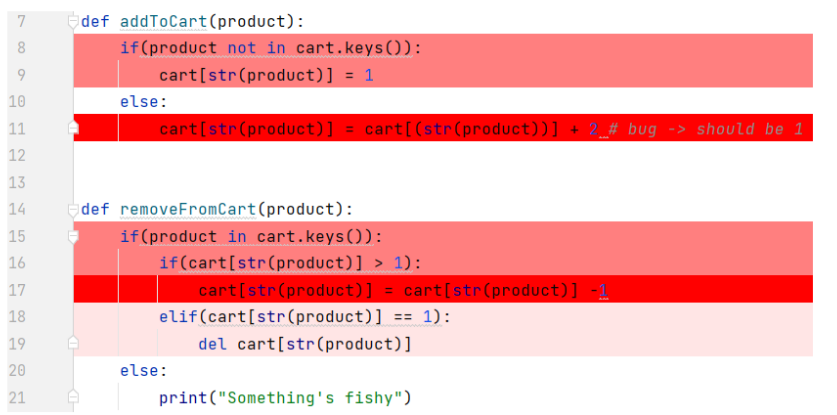
\includegraphics[width=10cm]{CharmFL.png}
		\caption{\label{fig:charmfl} Example interface of CharmFL \cite{sarhan2021charmfl}}
	\end{center}
\end{figure}

\section{Usability and Accessibility}
\label{sec:usability_accessibility}

Considering that the focus of AFLuent is not to simply be a fault localization
tool but rather an accessible one for beginner and novice developers, it's
important to better understand how the tool can be catered to that audience.
This can be done in many different ways, one of which is to increase the clarity
and verbosity of output messages from the tool. Instead of simply displaying the
ranked scores of statements, it would be more user friendly to explain the
meaning of the output to guide the user into beginning the debugging process.
Kohn \cite{kohn2019error} explores the experience of beginners with Python errors
with different severity and various Python interpreter error output. The results
confirm that more clear error messages tend to have a higher percentage of
students finding and fixing the error. This connection between error output and
the ability for beginner developers to fix faults is very crucial in the case of
AFLuent. And while a user survey is out of scope of this research, Kohn
provides encouragement to account for the different use cases in AFLuent and
attempts to provide a clear output that describes the fault and guides the
developer for the next step.

Another aspiration of AFLuent is to assist beginners in debugging their code in
ways that go beyond simply looking at the suspiciousness ranking of elements. By
identifying popular python errors in Python among beginners, cause of faults can
more quickly be pointed out after statement ranking has been produced. These
steps require additional analysis of the suspicious statements by analyzing
their syntax to identify potential causes. The goal of AFLuent would then become
more than simply locating the fault, but also giving an educated guess regarding
the reason behind the error. Cosman et al. \cite{cosman2020pablo} create a tool
named PABLO that uses a trained classifier to identify common bugs and faults in
beginner written Python programs. PABLO is also evaluated using an empirical and
human study to analyze how accurate it is in detecting mistakes and how helpful
users find the tool. Overall, PABLO is found to be ``helpful, providing
high-accuracy fault localization that implicates the correct terms
59-77\% of the time''. The ability of PABLO to describe the cause of error is
very valuable to incorporate in AFLuent, especially that AFLuent is only able to
conclude that there is an error and where it's possibly located. PABLO provides
another layer of fault localization that can only enhance the user experience.
